\documentclass[twoside]{book}

% Packages required by doxygen
\usepackage{fixltx2e}
\usepackage{calc}
\usepackage{doxygen}
\usepackage[export]{adjustbox} % also loads graphicx
\usepackage{graphicx}
\usepackage[utf8]{inputenc}
\usepackage{makeidx}
\usepackage{multicol}
\usepackage{multirow}
\PassOptionsToPackage{warn}{textcomp}
\usepackage{textcomp}
\usepackage[nointegrals]{wasysym}
\usepackage[table]{xcolor}

% Font selection
\usepackage[T1]{fontenc}
\usepackage[scaled=.90]{helvet}
\usepackage{courier}
\usepackage{amssymb}
\usepackage{sectsty}
\renewcommand{\familydefault}{\sfdefault}
\allsectionsfont{%
  \fontseries{bc}\selectfont%
  \color{darkgray}%
}
\renewcommand{\DoxyLabelFont}{%
  \fontseries{bc}\selectfont%
  \color{darkgray}%
}
\newcommand{\+}{\discretionary{\mbox{\scriptsize$\hookleftarrow$}}{}{}}

% Page & text layout
\usepackage{geometry}
\geometry{%
  a4paper,%
  top=2.5cm,%
  bottom=2.5cm,%
  left=2.5cm,%
  right=2.5cm%
}
\tolerance=750
\hfuzz=15pt
\hbadness=750
\setlength{\emergencystretch}{15pt}
\setlength{\parindent}{0cm}
\setlength{\parskip}{3ex plus 2ex minus 2ex}
\makeatletter
\renewcommand{\paragraph}{%
  \@startsection{paragraph}{4}{0ex}{-1.0ex}{1.0ex}{%
    \normalfont\normalsize\bfseries\SS@parafont%
  }%
}
\renewcommand{\subparagraph}{%
  \@startsection{subparagraph}{5}{0ex}{-1.0ex}{1.0ex}{%
    \normalfont\normalsize\bfseries\SS@subparafont%
  }%
}
\makeatother

% Headers & footers
\usepackage{fancyhdr}
\pagestyle{fancyplain}
\fancyhead[LE]{\fancyplain{}{\bfseries\thepage}}
\fancyhead[CE]{\fancyplain{}{}}
\fancyhead[RE]{\fancyplain{}{\bfseries\leftmark}}
\fancyhead[LO]{\fancyplain{}{\bfseries\rightmark}}
\fancyhead[CO]{\fancyplain{}{}}
\fancyhead[RO]{\fancyplain{}{\bfseries\thepage}}
\fancyfoot[LE]{\fancyplain{}{}}
\fancyfoot[CE]{\fancyplain{}{}}
\fancyfoot[RE]{\fancyplain{}{\bfseries\scriptsize Generated by Doxygen }}
\fancyfoot[LO]{\fancyplain{}{\bfseries\scriptsize Generated by Doxygen }}
\fancyfoot[CO]{\fancyplain{}{}}
\fancyfoot[RO]{\fancyplain{}{}}
\renewcommand{\footrulewidth}{0.4pt}
\renewcommand{\chaptermark}[1]{%
  \markboth{#1}{}%
}
\renewcommand{\sectionmark}[1]{%
  \markright{\thesection\ #1}%
}

% Indices & bibliography
\usepackage{natbib}
\usepackage[titles]{tocloft}
\setcounter{tocdepth}{3}
\setcounter{secnumdepth}{5}
\makeindex

% Hyperlinks (required, but should be loaded last)
\usepackage{ifpdf}
\ifpdf
  \usepackage[pdftex,pagebackref=true]{hyperref}
\else
  \usepackage[ps2pdf,pagebackref=true]{hyperref}
\fi
\hypersetup{%
  colorlinks=true,%
  linkcolor=blue,%
  citecolor=blue,%
  unicode%
}

% Custom commands
\newcommand{\clearemptydoublepage}{%
  \newpage{\pagestyle{empty}\cleardoublepage}%
}

\usepackage{caption}
\captionsetup{labelsep=space,justification=centering,font={bf},singlelinecheck=off,skip=4pt,position=top}

%===== C O N T E N T S =====

\begin{document}

% Titlepage & ToC
\hypersetup{pageanchor=false,
             bookmarksnumbered=true,
             pdfencoding=unicode
            }
\pagenumbering{alph}
\begin{titlepage}
\vspace*{7cm}
\begin{center}%
{\Large Projeto 1 de Programação Avançada }\\
\vspace*{1cm}
{\large Generated by Doxygen 1.8.13}\\
\end{center}
\end{titlepage}
\clearemptydoublepage
\pagenumbering{roman}
\tableofcontents
\clearemptydoublepage
\pagenumbering{arabic}
\hypersetup{pageanchor=true}

%--- Begin generated contents ---
\chapter{Projeto 1}
\label{md__r_e_a_d_m_e}
\Hypertarget{md__r_e_a_d_m_e}
Projeto 1 da disciplina D\+C\+A0202 -\/ Programação avançada , referente a primeira parte da avaliação da segunda unidade. 
\chapter{Hierarchical Index}
\section{Class Hierarchy}
This inheritance list is sorted roughly, but not completely, alphabetically\+:\begin{DoxyCompactList}
\item \contentsline{section}{poligono}{\pageref{classpoligono}}{}
\begin{DoxyCompactList}
\item \contentsline{section}{retangulo}{\pageref{classretangulo}}{}
\end{DoxyCompactList}
\item \contentsline{section}{ponto}{\pageref{classponto}}{}
\end{DoxyCompactList}

\chapter{Class Index}
\section{Class List}
Here are the classes, structs, unions and interfaces with brief descriptions\+:\begin{DoxyCompactList}
\item\contentsline{section}{\hyperlink{classpoligono}{poligono} }{\pageref{classpoligono}}{}
\item\contentsline{section}{\hyperlink{classponto}{ponto} }{\pageref{classponto}}{}
\item\contentsline{section}{\hyperlink{classretangulo}{retangulo} }{\pageref{classretangulo}}{}
\end{DoxyCompactList}

\chapter{Class Documentation}
\hypertarget{classpoligono}{}\section{poligono Class Reference}
\label{classpoligono}\index{poligono@{poligono}}
Inheritance diagram for poligono\+:\begin{figure}[H]
\begin{center}
\leavevmode
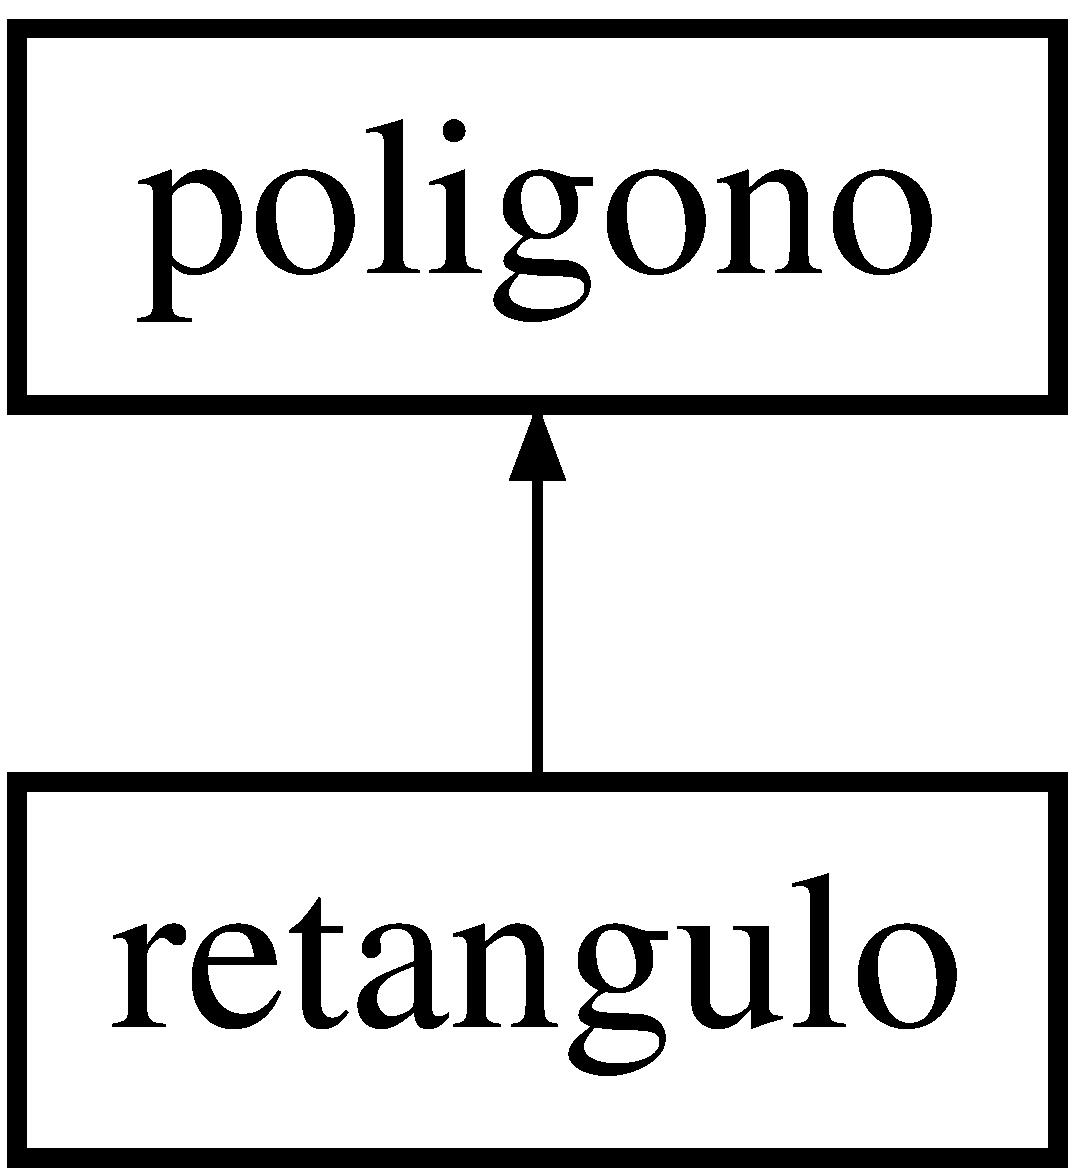
\includegraphics[height=2.000000cm]{classpoligono}
\end{center}
\end{figure}
\subsection*{Public Member Functions}
\begin{DoxyCompactItemize}
\item 
\mbox{\Hypertarget{classpoligono_a21b52ae5f6df8800e6249cb0936d63cf}\label{classpoligono_a21b52ae5f6df8800e6249cb0936d63cf}} 
{\bfseries poligono} (\hyperlink{classponto}{ponto} vetp\mbox{[}$\,$\mbox{]}, int t)
\item 
\mbox{\Hypertarget{classpoligono_a5358c8e540b968f4d2b229d7e7893896}\label{classpoligono_a5358c8e540b968f4d2b229d7e7893896}} 
void {\bfseries set\+Vertice} (\hyperlink{classponto}{ponto} ponto\+Novo)
\item 
\mbox{\Hypertarget{classpoligono_a6966febfd0e3eaebfb31a94b86cbf78b}\label{classpoligono_a6966febfd0e3eaebfb31a94b86cbf78b}} 
int {\bfseries get\+Vertices} ()
\item 
\mbox{\Hypertarget{classpoligono_a6f71f348af871870f02fcc15e506c240}\label{classpoligono_a6f71f348af871870f02fcc15e506c240}} 
float {\bfseries area} ()
\item 
\mbox{\Hypertarget{classpoligono_af4220ccf36d04de8b23ad3b956804a19}\label{classpoligono_af4220ccf36d04de8b23ad3b956804a19}} 
void {\bfseries translada\+Poligono} (int pos1, int pos1Y)
\item 
\mbox{\Hypertarget{classpoligono_a8b4a4a55f8488305a04f8c967b0dc8bf}\label{classpoligono_a8b4a4a55f8488305a04f8c967b0dc8bf}} 
void {\bfseries imprime} ()
\item 
\mbox{\Hypertarget{classpoligono_acdf2c4530d4964e3c004b42dd0e6996e}\label{classpoligono_acdf2c4530d4964e3c004b42dd0e6996e}} 
void {\bfseries rotaciona} (float angulo, \hyperlink{classponto}{ponto} ponto\+Pos)
\end{DoxyCompactItemize}


The documentation for this class was generated from the following files\+:\begin{DoxyCompactItemize}
\item 
poligono.\+h\item 
poligono.\+cpp\end{DoxyCompactItemize}

\hypertarget{classponto}{}\section{ponto Class Reference}
\label{classponto}\index{ponto@{ponto}}
\subsection*{Public Member Functions}
\begin{DoxyCompactItemize}
\item 
\mbox{\Hypertarget{classponto_a6d6d40e6c14e903c65c48988b65fb649}\label{classponto_a6d6d40e6c14e903c65c48988b65fb649}} 
{\bfseries ponto} (float \+\_\+x, float \+\_\+y)
\item 
\mbox{\Hypertarget{classponto_a64ff8ce435f3626995f535671a21403d}\label{classponto_a64ff8ce435f3626995f535671a21403d}} 
void {\bfseries setX} (float \+\_\+x)
\item 
\mbox{\Hypertarget{classponto_acf9918cb8a31b1f74e7425acee366322}\label{classponto_acf9918cb8a31b1f74e7425acee366322}} 
void {\bfseries setY} (float \+\_\+y)
\item 
\mbox{\Hypertarget{classponto_a29ac118d16c126d9d13ae8daff2f13cf}\label{classponto_a29ac118d16c126d9d13ae8daff2f13cf}} 
void {\bfseries set\+XY} (float \+\_\+x, float \+\_\+y)
\item 
\mbox{\Hypertarget{classponto_a72028c7500c56c02b7574ca2cff8a6b2}\label{classponto_a72028c7500c56c02b7574ca2cff8a6b2}} 
float {\bfseries getX} ()
\item 
\mbox{\Hypertarget{classponto_a880c3bd815e15edd0130c77d33a57c7c}\label{classponto_a880c3bd815e15edd0130c77d33a57c7c}} 
float {\bfseries getY} ()
\item 
\mbox{\Hypertarget{classponto_abbb3e8c2c0c74fba6c52e1b2c5ebfb76}\label{classponto_abbb3e8c2c0c74fba6c52e1b2c5ebfb76}} 
\hyperlink{classponto}{ponto} {\bfseries add} (\hyperlink{classponto}{ponto} p1)
\item 
\mbox{\Hypertarget{classponto_ac2e219ffd3a478a4326792452c0af734}\label{classponto_ac2e219ffd3a478a4326792452c0af734}} 
\hyperlink{classponto}{ponto} {\bfseries sub} (\hyperlink{classponto}{ponto} p1)
\item 
\mbox{\Hypertarget{classponto_ab0c5fb0ddcd79fdb70fefe4cb6d7360e}\label{classponto_ab0c5fb0ddcd79fdb70fefe4cb6d7360e}} 
float {\bfseries norma} ()
\item 
\mbox{\Hypertarget{classponto_a57873357b3df1ba47a54119d9a044a8e}\label{classponto_a57873357b3df1ba47a54119d9a044a8e}} 
void {\bfseries translada} (float a, float b)
\item 
\mbox{\Hypertarget{classponto_adf55fab25fa59c8a688eb1a1011eb2ae}\label{classponto_adf55fab25fa59c8a688eb1a1011eb2ae}} 
void {\bfseries imprime} ()
\end{DoxyCompactItemize}
\subsection*{Public Attributes}
\begin{DoxyCompactItemize}
\item 
\mbox{\Hypertarget{classponto_a5ab2f6400e904f54dabfffe45b3001df}\label{classponto_a5ab2f6400e904f54dabfffe45b3001df}} 
float {\bfseries x}
\item 
\mbox{\Hypertarget{classponto_a6c2bb55c1dabf042c072426759d33f40}\label{classponto_a6c2bb55c1dabf042c072426759d33f40}} 
float {\bfseries y}
\end{DoxyCompactItemize}


The documentation for this class was generated from the following files\+:\begin{DoxyCompactItemize}
\item 
ponto.\+h\item 
ponto.\+cpp\end{DoxyCompactItemize}

\hypertarget{classretangulo}{}\section{retangulo Class Reference}
\label{classretangulo}\index{retangulo@{retangulo}}
Inheritance diagram for retangulo\+:\begin{figure}[H]
\begin{center}
\leavevmode
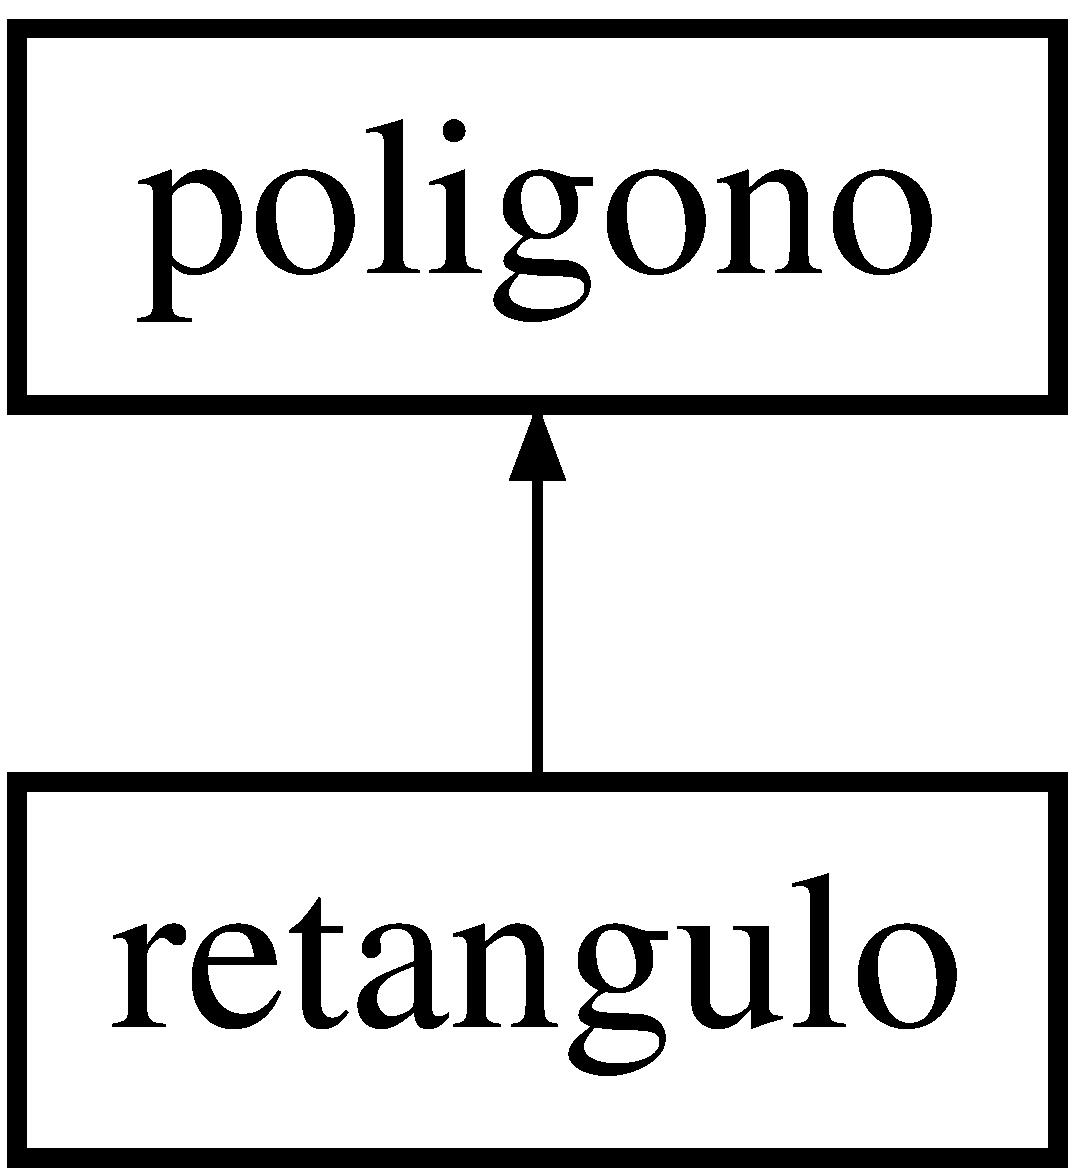
\includegraphics[height=2.000000cm]{classretangulo}
\end{center}
\end{figure}
\subsection*{Public Member Functions}
\begin{DoxyCompactItemize}
\item 
\mbox{\Hypertarget{classretangulo_ae4798266f2ab4b22ab5c90538d2f325e}\label{classretangulo_ae4798266f2ab4b22ab5c90538d2f325e}} 
{\bfseries retangulo} (float x\+\_\+, float y\+\_\+, float altura, float largura)
\item 
\mbox{\Hypertarget{classretangulo_a85473f314a045e4660e4441e6fd094a2}\label{classretangulo_a85473f314a045e4660e4441e6fd094a2}} 
void {\bfseries set\+XR} (float \+\_\+x)
\item 
\mbox{\Hypertarget{classretangulo_a537fa77cb92b402d8813eb4c07f7ac4a}\label{classretangulo_a537fa77cb92b402d8813eb4c07f7ac4a}} 
void {\bfseries set\+YR} (float \+\_\+y)
\item 
\mbox{\Hypertarget{classretangulo_a4a45f92c2a786cab5d7d51624f733273}\label{classretangulo_a4a45f92c2a786cab5d7d51624f733273}} 
void {\bfseries set\+Largura} (float largura)
\item 
\mbox{\Hypertarget{classretangulo_a5b21ff5724a23f455bcec0e405d96185}\label{classretangulo_a5b21ff5724a23f455bcec0e405d96185}} 
void {\bfseries set\+Altura} (float altura)
\item 
\mbox{\Hypertarget{classretangulo_a8e6a38a265c3ad1d80ab7f4917c149c5}\label{classretangulo_a8e6a38a265c3ad1d80ab7f4917c149c5}} 
float {\bfseries get\+XR} ()
\item 
\mbox{\Hypertarget{classretangulo_a74963fa0d52e94181142cceb460db188}\label{classretangulo_a74963fa0d52e94181142cceb460db188}} 
float {\bfseries get\+YR} ()
\item 
\mbox{\Hypertarget{classretangulo_aaafb6b2830fd492f5622ec7501aaf684}\label{classretangulo_aaafb6b2830fd492f5622ec7501aaf684}} 
float {\bfseries get\+Largura} ()
\item 
\mbox{\Hypertarget{classretangulo_ab7f54ba43a0def6ba98497654792a11d}\label{classretangulo_ab7f54ba43a0def6ba98497654792a11d}} 
float {\bfseries get\+Altura} ()
\end{DoxyCompactItemize}
\subsection*{Public Attributes}
\begin{DoxyCompactItemize}
\item 
\mbox{\Hypertarget{classretangulo_addf35a5b55900206b425986c28174469}\label{classretangulo_addf35a5b55900206b425986c28174469}} 
float {\bfseries x1}
\item 
\mbox{\Hypertarget{classretangulo_a37160bd3fb59f4c4c12525ac7b94678e}\label{classretangulo_a37160bd3fb59f4c4c12525ac7b94678e}} 
float {\bfseries y1}
\item 
\mbox{\Hypertarget{classretangulo_a977ab31fc5998d9e42c94f62a6c68b71}\label{classretangulo_a977ab31fc5998d9e42c94f62a6c68b71}} 
float {\bfseries larg}
\item 
\mbox{\Hypertarget{classretangulo_a72b730a7156f944fa3b1d4edff1cbe0d}\label{classretangulo_a72b730a7156f944fa3b1d4edff1cbe0d}} 
float {\bfseries alt}
\end{DoxyCompactItemize}


The documentation for this class was generated from the following files\+:\begin{DoxyCompactItemize}
\item 
retangulo.\+h\item 
retangulo.\+cpp\end{DoxyCompactItemize}

%--- End generated contents ---

% Index
\backmatter
\newpage
\phantomsection
\clearemptydoublepage
\addcontentsline{toc}{chapter}{Index}
\printindex

\end{document}
